\chapter{BACKGROUND}
\label{chap-two} 

\section{Human Brain}
	The Human Brain is an important part of the human nervous system. Along with spinal chord, the brain, as part of central nervous system, is analogous to Central processing unit (CPU) of a computer. The human brain is mostly composed of neurons which are electrically excitable cells, blood vessels and glial cells. Neurons can transmit information through electrical and chemical signals. The human brain is interconnected with following three major components,
    \begin{enumerate}
		\item Brain Stem
        \item Cerebellum
        \item Cerebrum
	\end{enumerate}


    \begin{figure}[hbtp]
    	\centering
    	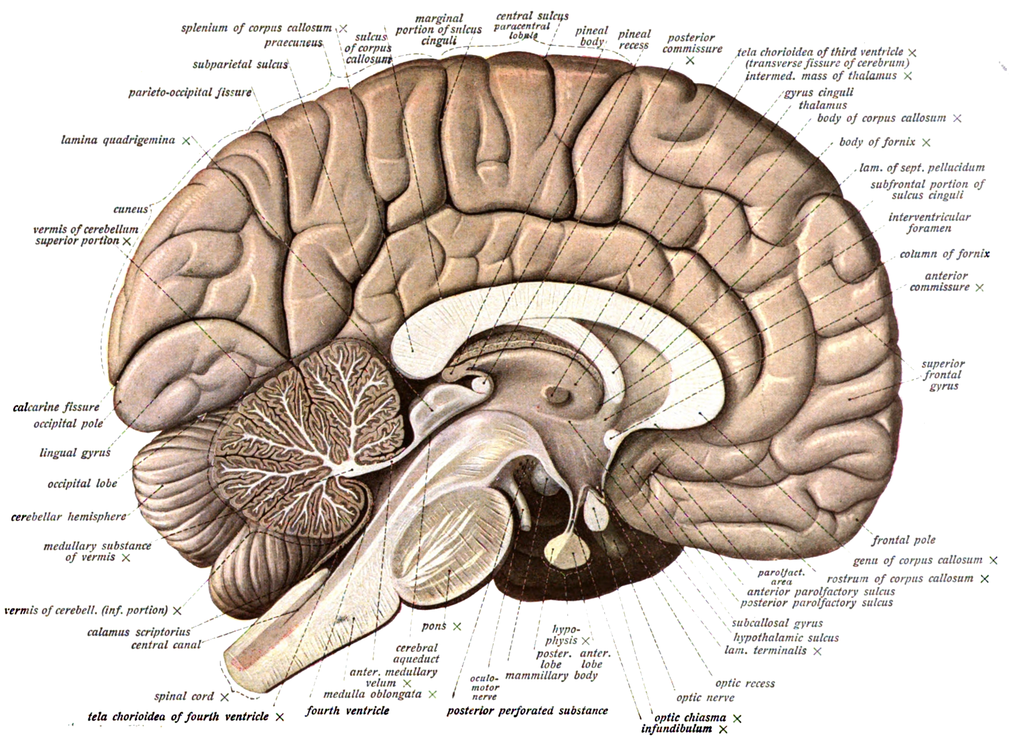
\includegraphics[width=1\textwidth]{Chapter-2/Human_brain}
    	\caption{The Human Brain (Mid-line incision view) \cite{JohannesSobotta}}
    	\label{fig:brain}
  	\end{figure}
    
	\subsection{Brain Stem}
        The Brain stem connects the brain to the spinal cord and also controls autonomic processes like breathing, digestion and heart rate.

	\subsection{Cerebellum} 
        	The Cerebellum plays an important role in balance and motor control, but is also involved in some cognitive functions such as attention, language, emotional functions and in processing and storage of memories.

 	\subsection{Cerebrum}
    	The Cerebrum is divided into two hemispheres (left and right) by the longitudinal fissure. It is also covered with a layer of neural tissues known as the Cerebral Cortex which envelops organs like thalamus, hypothalamus and pituitary glands. The Thalamus helps in relying information from the brain stem and the spinal cord to the cerebral cortex. The hypothalamus and the pituitary glands control visceral functions, body temperature and behavioral responses.  The Cerebral Cortex plays key role in memory, attention, thought, awareness, language and consciousness.
        
\section{Electroencephalography (EEG)}
\label{Electroencephalography (EEG)}
	Understanding how the brain works is a necessity in order to find solutions for various brain disorders like epilepsy, dementia, tumor etc. The methods to study the brain can be broadly classified into two methods,
    \begin{enumerate}
		\item An Invasive Approach - Requires physical implant of electrodes inside the brain.
        \item A Non-Invasive Approach - Include methods like Magnetic Resonance Imaging(MRI) and Electroencephalography.
	\end{enumerate}
    According to \cite{Kropotov}, both the methods give different perspectives and enable us to look inside the brain and observe what happens.
    
    
    Electroencephalography (EEG) was invented by a German psychiatrist, Hans Berger, who also coined the term ``Electroencephalography''. An EEG is, as defined by the Mayo Clinic, ``A test that detects electrical activity in your brain using small, flat metal discs (electrodes) attached to your scalp'' . In a healthy human brain, the brain cells (neurons), are active all the time, even while resting. As the result of these neural activities, electrical impulses are produced. What we call ``thought'' is in fact ever an changing symphony of such electrical impulses. The rhythmic neural activity in the central nervous system is popularly known as \textit{Neural Oscillation} or \textit{Brain Waves}.  For a given neuron these oscillation can occur due to rhythmic changes in the membrane potential. When these oscillations occur synchronously in a large group of neurons, macroscopic oscillations can easily be captured by EEG devices.

\section{Pattern Recognition}
	According to Charles W. Therrien \cite{Therrien:1989:DEC:61950}, `` The goal of pattern recognition is to classify objects of interest into one of a number of categories or \textit{classes}. The objects of interest are generally called \textit{patterns}''. The data used to discover the patterns is called the \textit{Training set}. The data on which the predicted pattern is tested is called the \textit{Testing set}. Pattern recognition can fall into one of the following two types,
    
    \begin{enumerate}
		\item \textbf{Supervised Pattern recognition:} If the classes of training set are known beforehand.
        \item \textbf{Unsupervised Pattern recognition or clustering:} If the classes of the training set and maybe even number the of classes are unknown before hand.
	\end{enumerate}
    
    A typical pattern recognition system is shown in Figure \ref{fig:pattern_pipeline}.
    \begin{figure}[hbtp]
        \centering
        \smartdiagram[priority descriptive diagram]{
            \centering
            Sensor,
            Pre-processing,
            Feature Extraction,
            Classifier,
            Class Assignment}
        \caption{A typical pattern recognition system}
        \label{fig:pattern_pipeline}
    \end{figure}

    
\section{Electroencephalography Sensors}
\label{Electroencephalography Sensors}
	In EEG sensors the voltage fluctuation due to the brain waves are read from the sensitive electrodes attached to the scalp. When neurons are electrically charged, electrons are either pushed to these electrodes or pulled from the electrodes and the voltage difference between any of two such electrodes can be measured by a voltmeter. Hence, EEG sensors will typically have a ground electrode, a system reference electrode along with one or more recording electrodes. In 1958, International Federation in Electroencephalography and Clinical Neurophysiology adopted standardization for electrode placement called 10-20 electrode placement system \cite{H.H.Jasper} (see Figure \ref{fig:standard}).

	There are different types of EEG sensors available, some are sophisticated and used in labs for advance research. Some sensors are available for commercial use. Notable ones are EPOC from Emotive, MUSE and MindWave from NeuroSky. More details about the commercial EEG sensors are discussed in Section \ref{Commercial EEG sensors}.

  \begin{figure}[hbtp]
    \centering
    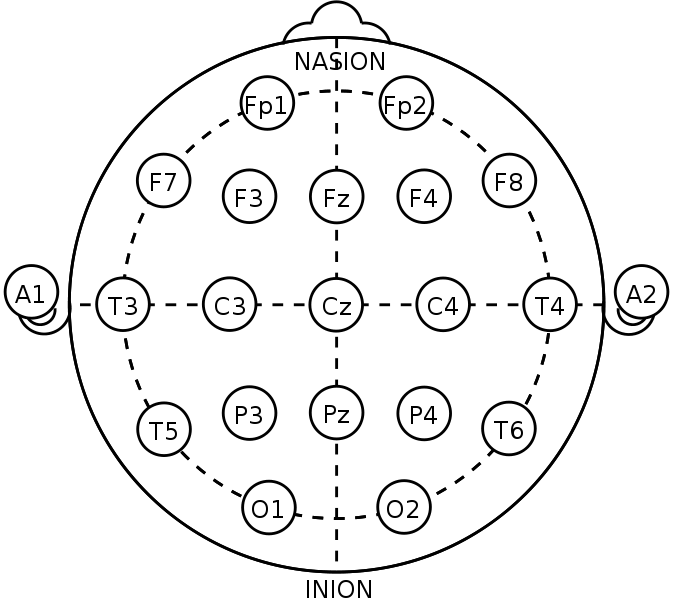
\includegraphics[width=1\textwidth]{Chapter-2/Standard}
    \caption{The 1020 System - Standardized placement of electrodes on scalp for EEG
    measurements \cite{system1020}}
    \label{fig:standard}
  \end{figure}

    \section{Raw EEG Data}
    	When an electrode in an EEG device captures the electrical activity (which occurs due to the neural activities), it also captures the electrical activity in its proximity. The captured signal also known as ``Raw EEG Data'', is a result of combination of the neural activities, electrical activity of nearby muscles and ambient noise. Generally, to reduce the effect of ambient noise, the Raw EEG Data is subjected to pre-processing methods which include digital filtering (discussed in Section \ref{Pre-processing Methods}). Also, different frequency of the raw EEG data can be linked to different brain activities. More details about EEG Frequency bands is discussed in Section \ref{EEG Frequency Bands}.
        
        
    \section{EEG Frequency Bands}
    \label{EEG Frequency Bands}
    
    The neural oscillations detected by the EEG sensors as discussed in Section \ref{Electroencephalography Sensors} are characterized by frequency, amplitude and phase. These characteristics can be extracted by time-frequency analysis. The important frequency bands associated with the brain waves are shown in the Table \ref{Table:Bands}.
    
	\begin{table}[h!]
		\centering
		\caption{EEG Frequency Bands}
		\label{Table:Bands}
		\begin{tabular}{l l}
			\hline
			Name &Frequency Band\\\hline
			Delta&0.1Hz - 4Hz\\
			Theta&4Hz - 8Hz\\
			Alpha&8Hz - 12Hz\\
			Beta&12Hz - 30Hz\\
			Gamma&30Hz - 48Hz\\
		\end{tabular}
	\end{table}

	\subsection{Delta}
    	Delta waves are low frequency waves (0.1Hz to 4Hz) generated by the brain when the individual is in deep sleep, non-REM sleep or unconscious. The delta waves are generally not detected if the individual is awake, if detected, it is either due to artificial delta waves created due to movements or due to defects in the brain.
        
	\subsection{Theta}
    	Theta waves range from 4Hz to 8Hz and are linked to Intuitive thinking, creative thinking, recall, fantasy and day dreaming. Theta waves can arise from emotional stress like frustration and disappointment \cite{YanZhang}. According to Heinrich et al.~\cite{H.H.Jasper} high level of Theta waves is considered abnormal among adults and possibly related to AD/HD.
        
	\subsection{Alpha}
    	Theta waves range from 8Hz to 12Hz and are associated with the state of relaxation while not drowsy, being tranquil and conscious.
    
    \subsection{Beta}
    	Beta waves range from 12Hz to 30Hz and are associated with performing integrative thinking, agitation, alertness, state of being relaxed yet focused and aware of self and surrounding. According to Y.Zang et al. \cite{YanZhang}, resisting or suppressing movement, or solving a math task, there is an increase of beta wave levels.
    
    \subsection{Gamma}
    	Gamma waves range from 30Hz to 48Hz and are associated with state of attention, perception, and cognition.

    \section{Commercial EEG sensors}
    \label{Commercial EEG sensors}
    Various EEG sensors are available in the market and many of them with sophisticated design are used by a doctor to examine a patient or for medical research. Figure \ref{fig:eeg_mesh} shows an example EEG sensor used in research \cite{EEGmesh}. Many EEG sensors are available for commercial use as well. EPOC from Emotive \cite{Emotive}, MUSE \cite{muse} and MindWave from NeuroSky \cite{MWMobile} are some of the notable ones.
    
	\begin{figure}[hbtp]
    	\centering
    	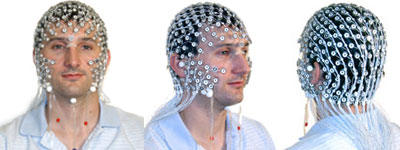
\includegraphics[width=0.9\textwidth]{Chapter-2/EEG_mesh}
    	\caption{A Geodesic Sensor Net \cite{EEGmesh}}
    	\label{fig:eeg_mesh}
  	\end{figure}
  
    	\subsection{Mindwave Mobile}
        	MindWave Mobile (shown in Figure \ref{fig:mindwavemobile}) is an EEG headset released by NeuroSky for commercial use \cite{MWMobile}. It has a recording sensor as part of the sensor arm which can be rested on forehead along with reference and ground sensors on the ear clip. The EEG data recorded from the sensors are transferred via Bluetooth to the Bluetooth enabled device like a Mac, a PC, an iPhone or an Android phone.
            
            \textbf{NOTE:} Along with the raw EEG data, MindWave Mobile can also transfer the brain wave frequency band readings, attention and meditation meters.
            
            The specifications of MindWave Mobile are as given in the Table \ref{specs}.
        \begin{table}[h!]
          \centering
          \caption{MindWave Mobile Specifications}
          \label{specs}
          \begin{tabular}{l l}
            \hline
            Parameters &Value\\\hline
            Raw EEG output & 3 to 100Hz\\
            Proprietary meters & Attention and Meditation\\
            EEG Power Spectrum & Delta, Alpha, Beta, Gamma\\
            Sampling Frequency & 512Hz\\
            Bluetooth Version&v2.1 Class 2\\
            Bluetooth Range &10m\\
            Bluetooth Pairing &Automatic\\
            Headset Type& Static\\
          \end{tabular}
        \end{table}
        
        \begin{figure}[hbtp]
            \centering
            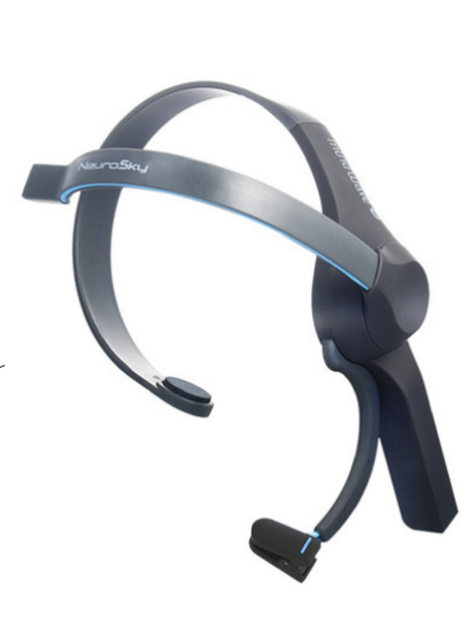
\includegraphics[width=0.9\textwidth]{Chapter-2/mindwavemobile}
            \caption{Mindwave mobile Sensor }
            \label{fig:mindwavemobile}
        \end{figure}
    
    
\section{Feature Extraction}
\label{Pre-processing Methods}
	Digital raw signal acquired from the EEG sensor are subjected to various pre-processing methods in order to extract features. These features are later used as the inputs to the classifiers. These features are generally the frequency spectrum energy bands shown in Table \ref{Table:Bands}. Multi-rate Filter banks and Fast Fourier Transform (FFT) can be used to extract the average magnitude of each spectral bands.
        
    \subsection{Fast Fourier Transforms(FFT)} 
    	The Fast Fourier Transforms (FFT) is an optimized and efficient algorithm to computer the Discrete Fourier Transform of a signal. Spectral energy of each EEG frequency band can then be calculated for each respective band of the FFT (additional details are presented in Section \ref{FeatureExtraction}).
   
\section{Classifier}
	The Classifier analyzes the feature vector (obtained by the passing prepossessed \textit{input pattern} or \textit{input vector} or \textit{measurement vector} through feature extractor) and assigns a class to the pattern. The classifier essentially induces a partitioning of the feature vector space into a number of disjoint regions \cite{Therrien:1989:DEC:61950}. Figure \ref{fig:regions} shows one such partition of the feature vector space. Here, if the feature vector falls in the region $R3$, class $c3$ is assigned to the corresponding input pattern.
    
		\begin{figure}[hbtp]
            \centering
            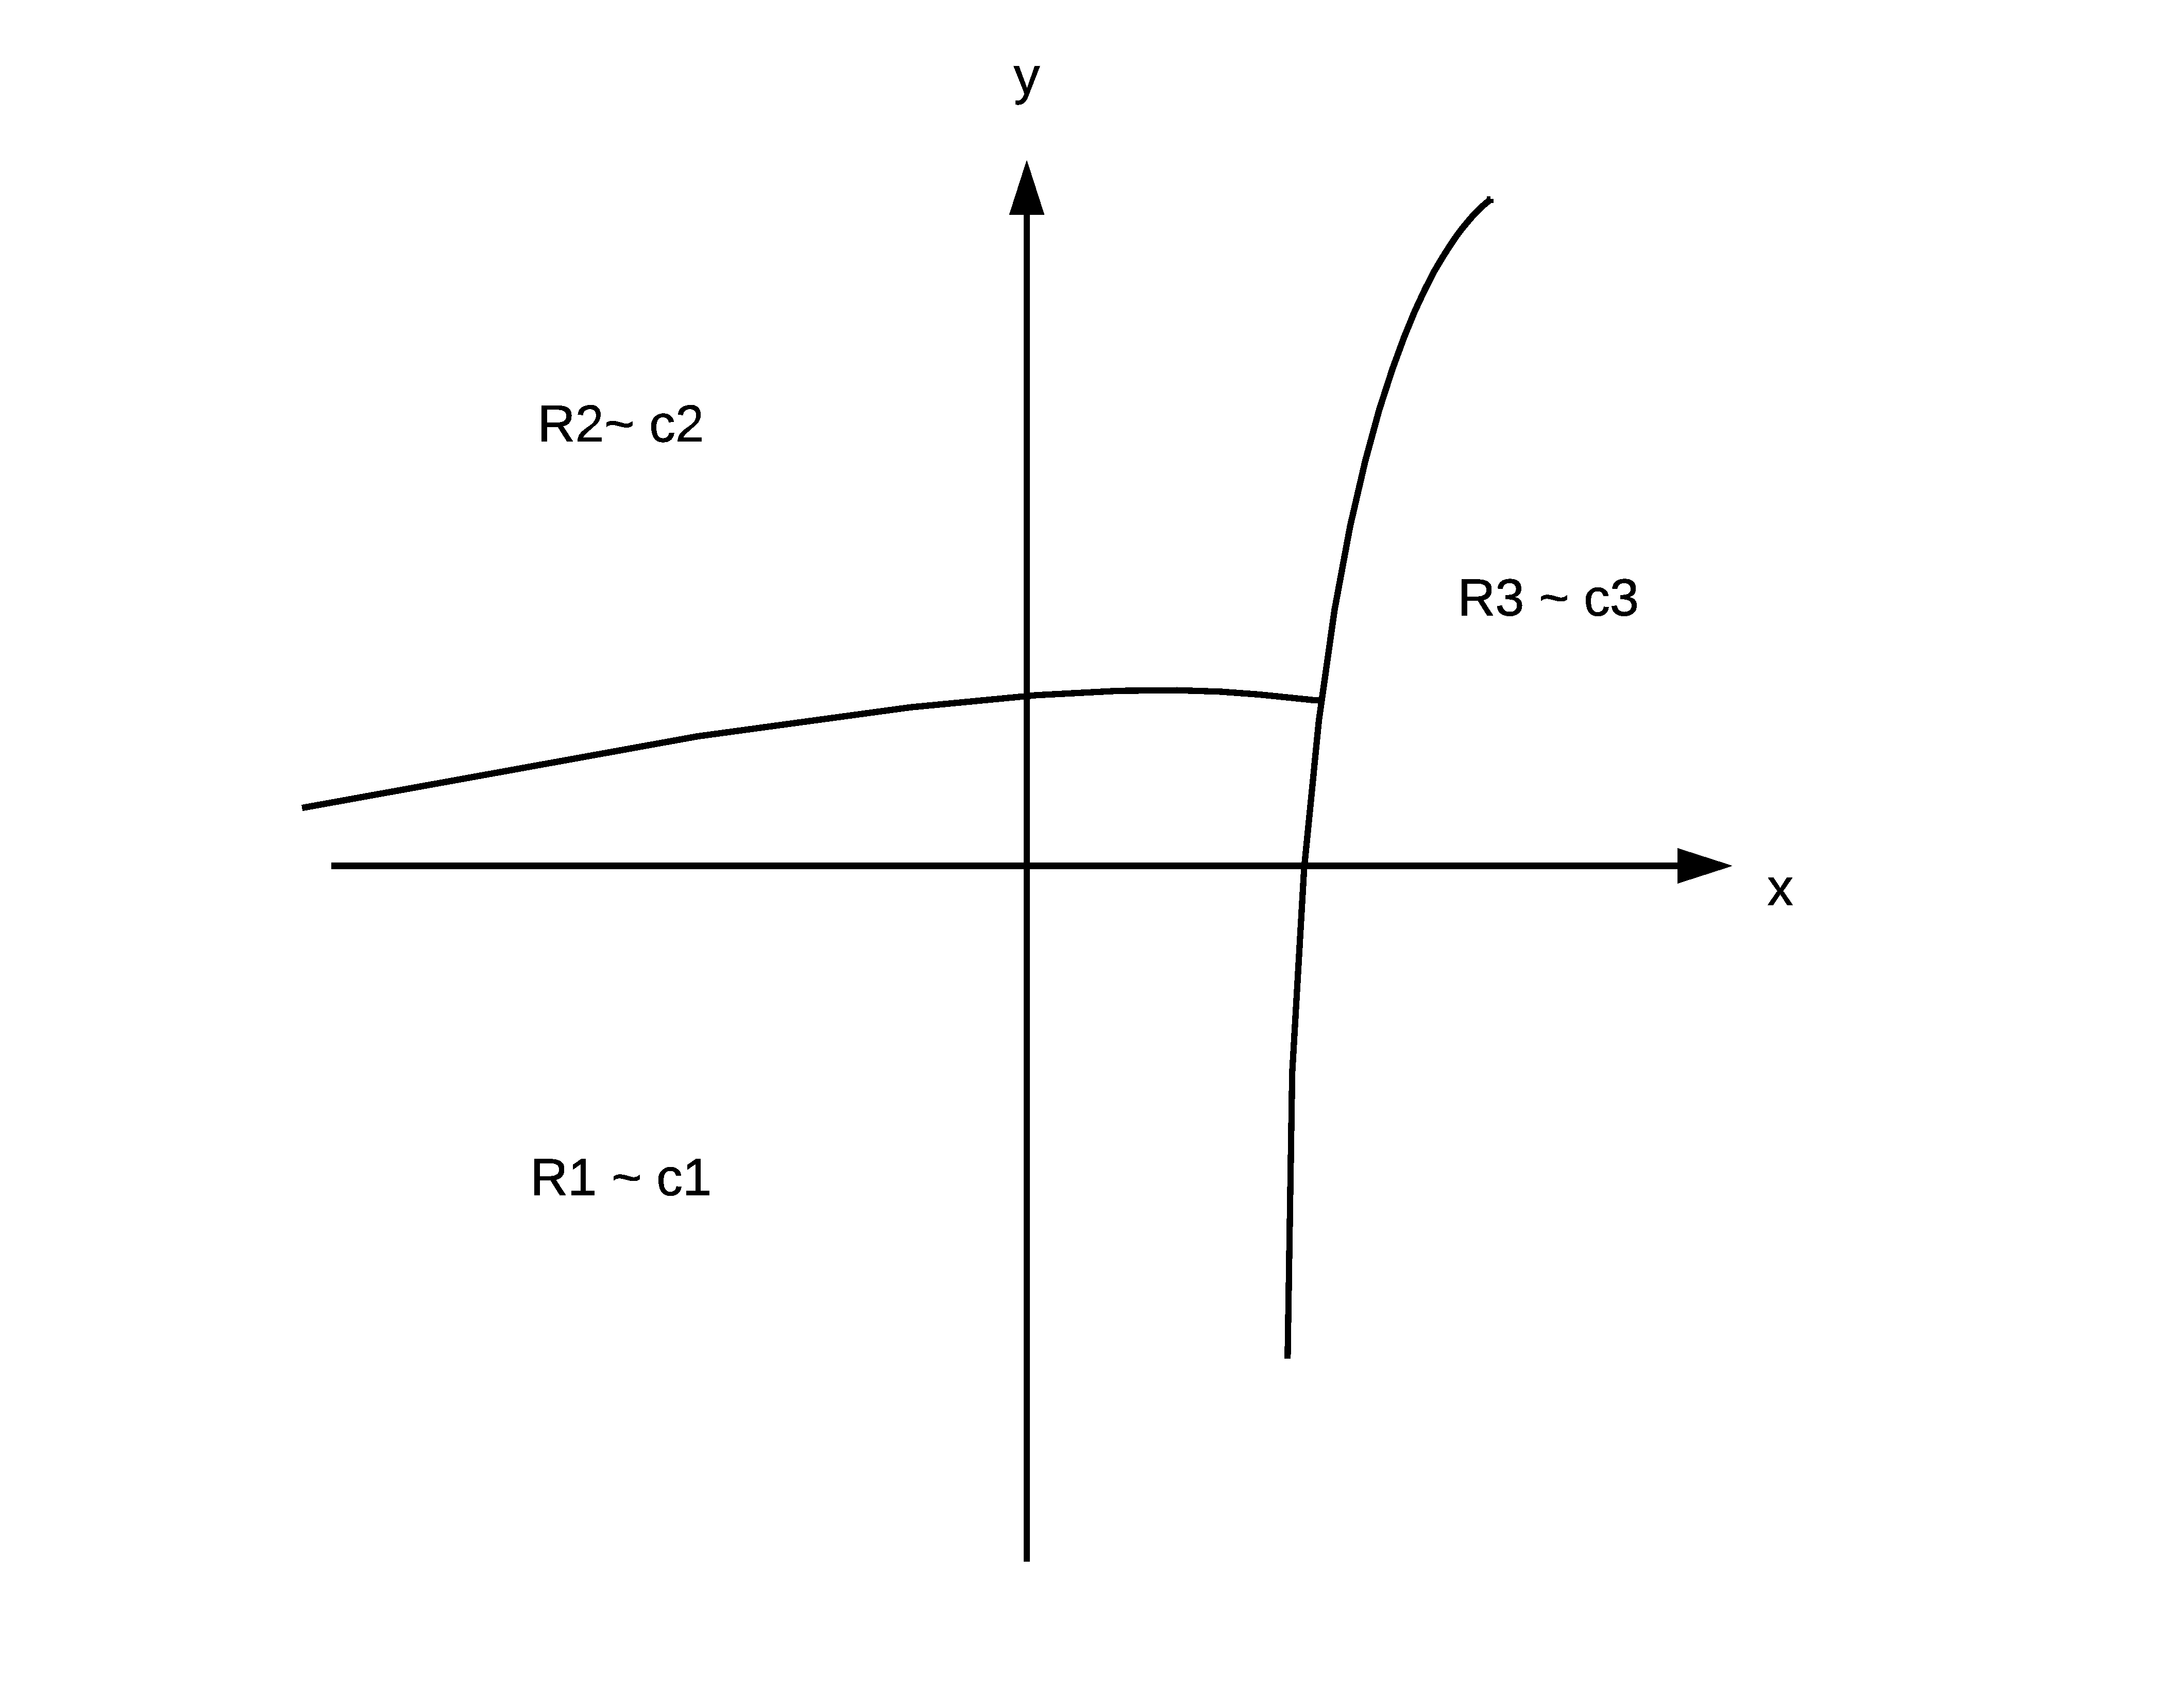
\includegraphics[width=0.9\textwidth]{Chapter-2/regions}
            \caption{Partition of feature space \cite{Therrien:1989:DEC:61950} }
            \label{fig:regions}
        \end{figure}
        
	\subsection{Mahalanobis Distance}
    \label{Chap2:Maha}
		The Mahalanobis Distance is one of the measures of distance between a feature vector and a class, it is given by Eq(\ref{Maha}).
        
		\begin{equation}
			D^2_x = (X - \mu)^T  \Sigma ^{-1}  (X - \mu)
			\label{Maha}
		\end{equation}
        
		where $D_x$ is the Mahalanobis distance, $X$ is the data vector, $\mu$ is estimated using $\mu = \frac{1}{n}\sum X$ over all the vectors in the class and $\Sigma$ is the covariance matrix of $X$. As we can see, the Mahalanobis distance is the argument of exponential of the multi-variate Gaussian Distribution that a given data vector (or feature vector) is a member of the set of vectors described by the Gaussian distribution with $\mu$ mean and $\Sigma$ covariance. \newline

		For each class $C_i$ of the training set, the mean vector $\mu_{C_i}$ and the covariance matrix $\Sigma_{C_i}$ are calculated. Using $\mu_{C_i}$ and $\Sigma_{C_i}$ of each class, the Mahalanobis Distances ($D_{XC_i}$) of the input vector $X$ in the testing set is calculated. The minimum Mahalanobis distance $D_{min}$ is then calculated using $D_{min} = min(D_{XC_i})$. The class to which the input vector $X$ belongs to is then determined by the class $C_i$ (with mean vector $\mu_{C_i}$ and the covariance matrix $\Sigma_{C_i}$) corresponding to the smallest Mahalanobis distance ($D_{min}$) for the input vector.
		
	\subsection{Artificial Neural Networks(ANN)}
    \label{Chap2:ANN}
		The Artificial Neural Networks are inspired by the behavior of biological neurons and are extensively used in machine learning field. A computational model for Neural Networks called \textit{threshold logic} was created by Warren McCulloch and Walter Pitts in 1943 \cite{McCulloch1943}. In 1958, Frank Rosenblatt created an algorithm called \textit{perceptron}, which could be used for pattern recognition \cite{Rosenblatt1958thePerceptron}. In 1975, Paul Werbos made one of the biggest advances in neural network research by creating the backpropagation algorithm \cite{werbos1974beyond}, which solved the exclusive-or issue faced by the perceptron algorithm. 
        
        An \textit{Artificial Neuron} is defined as a sum-of-products operator which produces a weighted sum of its inputs and passes it though a non-linear function such as a limiter or a sigmoid \cite{snyder2010machine} as shown in the Figure \ref{fig:ann}. An Artificial Neural Network (ANN) consists of several of such interconnected artificial neurons. A typical artificial neural network consists of an input layer, an output layer and single or many hidden layers as shown in Figure \ref{fig:nn}. Following are the types of Artificial Neural Networks.
        
        \begin{enumerate}
        	\item \textbf{Feedforward neural network -} Here the direction of data flow is from input layer to output layer and sigmoid activation is generally used.
            \item \textbf{Radial basis function network -} Here the hidden layers use Radial Basis Functions (usually Gaussian).
           	\item \textbf{Recurrent neural network -} Here the data flow can be bi-directional.
        \end{enumerate}
        
		\begin{figure}[hbtp]
			\centering
			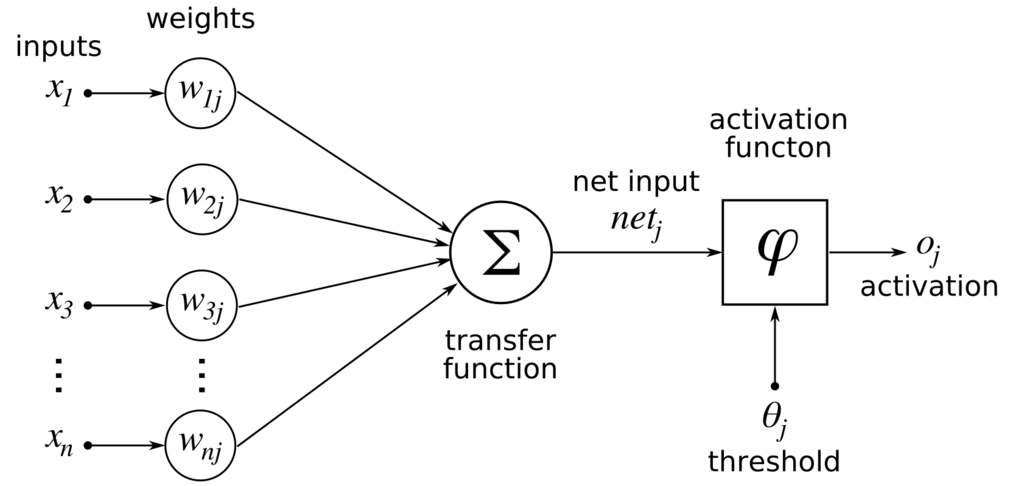
\includegraphics[width=0.9\textwidth]{Chapter-2/ann}
			\caption{An Artificial Neuron \cite{aneuronimage}}
			\label{fig:ann}
  		\end{figure}
        
        \begin{figure}[hbtp]
          \centering
          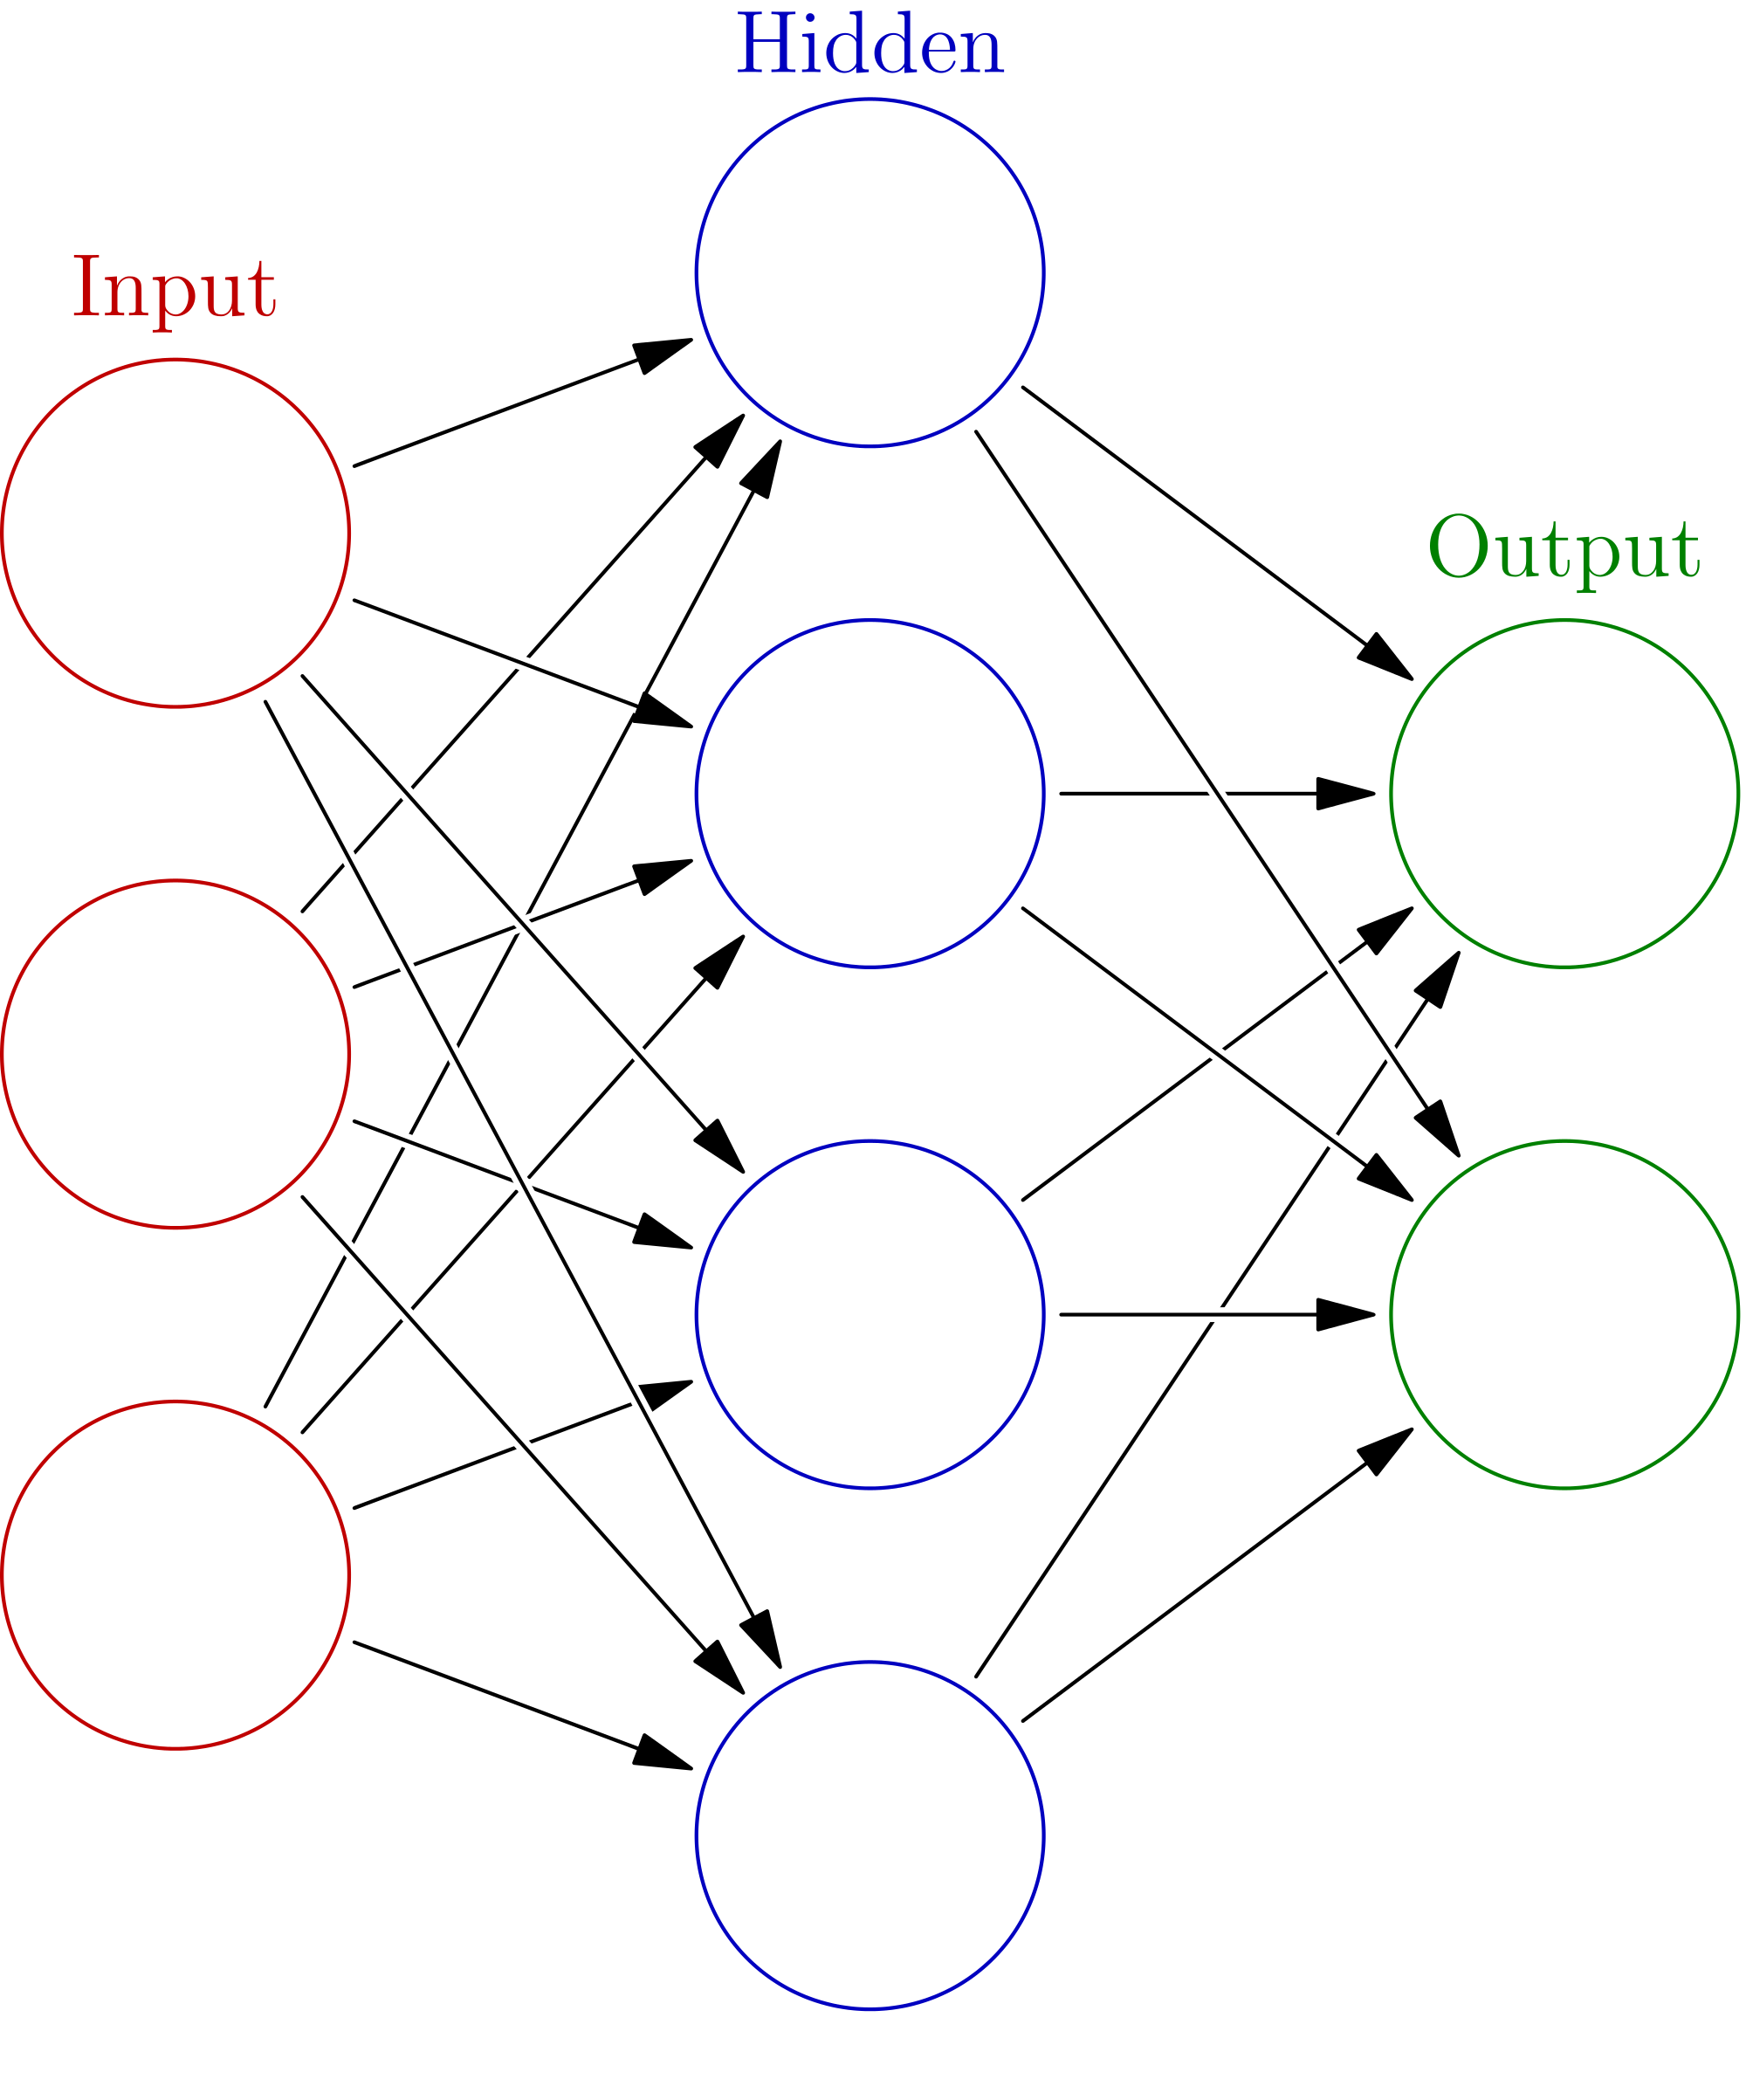
\includegraphics[width=0.6\textwidth]{Chapter-2/nn}
          \caption{A typical Artificial Neural Network with Input, Hidden and Output Layers\cite{nnimage}}
          \label{fig:nn}
  		\end{figure}
    
        In a typical feedforward neural network, the neurons in input layer are connected to the neurons in the first hidden layer and neurons in the first hidden layer are connected to the neurons in the second hidden layer and so on until the output layer. When the neural network is trained, the input activates the neurons of input layer and the activation propagates to the output layer. One of the algorithms used to train neural networks is \textit{Backpropagation} algorithm. It is an iterative algorithm which trains the neural network and adjusts the network parameters by minimizing the output error. More details about the Neural Networks and the backpropagation algorithm is discussed in Section \ref{Artificial Neural Networks}.

	\subsection{Support Vector Machines (SVM)}
    \label{chap2:SVM}
		The Support vector machines is one of the supervised learning models used in machine learning introduced by Vapnik \cite{Boser:1992:TAO:130385.130401}. The SVMs preprocess the m-dimensional input vector to represent patterns in a n-dimension space - typically $n>>m$. With an appropriate non-linear mapping function to a sufficiently higher dimension, data from two categories can be separated by a hyperplane \cite{duda2001pattern}. Say if we have class $C_1$ and $C_2$ which are separable by a hyperplane. Let, $d_1$ be the distance between closest point of $C_1$ and the hyperplane. Similarly, let $d_2$ be the distance between closest point of $C_2$ and the hyperplane. The \textit{margin} is defined as $d_1 + d_2$. Support Vector Machines can be seen as an optimization problem which minimize the margin \cite{snyder2010machine} (See Figure \ref{fig:badsvm} and Figure \ref{fig:goodsvm} for a non-optimal and an optimal choice of dividing hyperplane in 2D).
        
        \begin{figure}[hbtp]
            \centering
            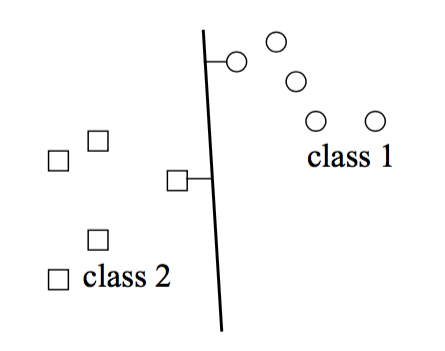
\includegraphics[width=0.6\textwidth]{Chapter-2/badsvm}
            \caption{Non-optimal dividing hyperplane \cite{snyder2010machine}}
            \label{fig:badsvm}
  		\end{figure}
        \begin{figure}[hbtp]
            \centering
            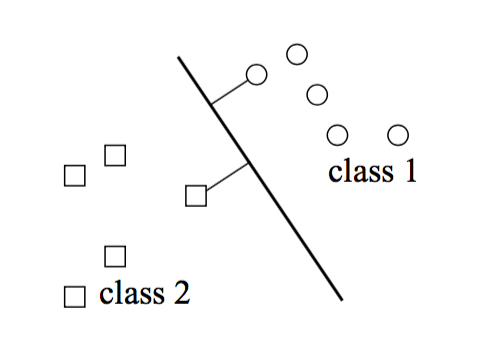
\includegraphics[width=0.6\textwidth]{Chapter-2/goodsvm}
            \caption{Optimal dividing hyperplane \cite{snyder2010machine}}
            \label{fig:goodsvm}
  		\end{figure} 
        
        Since SVMs deal with separating the input data into two by a hyperplane, it is suitable for binary classification, in fact, SVMs can be seen as a non-probabilistic binary linear classifiers. However, multi-class classification can be done by reducing the multi-class classification problem into many binary classification problems. For example, one-vs-rest or one-vs-all is one of the methods used for this. In one-vs-all classification method, a series of binary classifiers are built which distinguish between one class and the rest. The classes are then assigned using winner-take-it-all strategy. Section \ref{Support Vector Machines} discusses about the Support Vector Machines in greater detail.
        
        \section{Conclusion}
        	In Chapter \ref{chap-two}, we discussed about security, security typed, usage of EEG in security and methods used to achieve the same using pattern recognition methods. In Chapter \ref{chap-three}, we will discuss in more detail about the design and methodology of pattern recognition pipeline of a security system using EEG.
        